\section{UTXO-based cryptocurrencies}
\label{sec:concept_utxo}%


\begin{figure*}
  \centerline{%
    \ifdefined\varInputFigs%
    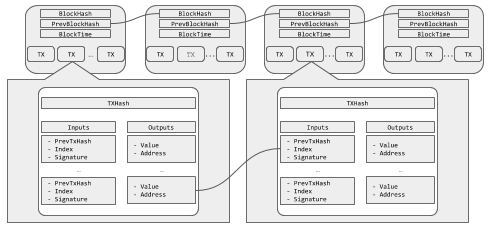
\includegraphics[width=0.8\linewidth]{fig/utxo_sys}%
    \else%
    \fi%
  }%
  \caption{Blockchain and Transactions (adapted from \cite{tschorsch2016bitcoin}).}
  \label{fig:utxo_sys}
\end{figure*}


Bitcoin builds its transaction graph chaining transaction outputs. %
This approach is followed by many altcoins, referred to as %
\emph{UTXO-based cryptocurrencies}. %
UTXO refers to the ``coins'' that can be spent---\emph{unspent transaction
  outputs}.%
\footnote{For a detailed explanation of UTXO-based and account-based %
  cryptocurrency systems see \cite{zahnentferner2018chimeric}.} %
Thus, UTXO-based cryptocurrencies record only transactions, in contrast to
account-based cryptocurrencies which store a balance for each address on
their blockchain. %
% (compare \cite{zahnentferner2018chimeric})
As an extensive exposition is provided by \cite{tschorsch2016bitcoin}, we
restrict ourselves to features relevant for calculating velocity measures. %

UTXO-based cryptocurrency protocols ensure an ordered transaction history
using a linked chain of so-called \textit{blocks} (compare
\reffig{utxo_sys}). %
These blocks contain a hash ({\ttfamily\bfseries\slshape BlockHash})
fingerprinting the information of all transactions recorded in the block, a
timestamp ({\ttfamily\bfseries\slshape BlockTime}) and the hash of the
previous block ({\ttfamily\bfseries\slshape PrevBlockHash}). %
This constellation of hashes and timestamps establishes pointers that are
determining the order of blocks. %
The process of creating new blocks, called \emph{mining}, creates new
monetary units in so called \emph{coinbase transactions}. %
Creating blocks usually involves solving a computationally demanding puzzle
(\emph{proof-of-work}) or proving stake in the existing coin supply
(\emph{proof-of-stake}). %

Generally, transactions contain a hash as identifier
({\ttfamily\bfseries\slshape TxHash}) as well as inputs and outputs. %
Coinbase transactions are exceptions as they include an output but no
input. %
This effectively increases the amount of spendable outputs, and thus money in
the system. %
% Fees can be paid to miners by constructing a transaction with a lower sum
% of output than input values. %
Inputs are recorded as links back to outputs of a previous transaction
identified by an index ({\ttfamily\bfseries\slshape PrevTxHash}). %
Outputs can be sent to addresses ({\ttfamily\bfseries\slshape Address})
corresponding to public keys of an appropriately generated public--private
key pair. %
Unspent previous outputs can be used as inputs only upon proving ownership
({\ttfamily\bfseries\slshape Signature}). %
Generating this proof requires the private key belonging to the public key
which received the output. %
Importantly, transaction inputs can only be spent as a whole. %
If a fraction of the input is to be retained, an additional output must be
included which links to an address belonging to the spender. %
Such addresses are known as \textit{change addresses} and we refer to the
respective outputs as \textit{change outputs}. %

We refer to all outputs sent to an address controlled by the sender,
following~\cite{kalodner2017blocksci}, as \emph{self-churn}. %
Since the concept of \textit{user identities} does not exist in UTXO-based
cryptocurrencies, there is no direct way to clearly separate self-churn from
outputs transferred to third parties \citep[cf.][]{meiklejohn2013fistful}. %
Moreover, no relation between elements of the set of inputs and those in the
set of outputs of a transaction is determined. %
In other words, no technical link between individual outputs and inputs
exists; unspent outputs are fully fungible. %
Therefore, velocity measures cannot be calculated by following ``coins'' or
UTXOs through their transactions: due to splitting and rejoining within
blocks there exists no ``path'' the money took.

% Mixing services make use of the unspecified assignment between inputs and
% outputs of a transactions to obfuscate the link between transactions even
% further.%
% \footnote{%
% 	This practice is sometimes referred as \textit{coinjoins} where money from %
% 	different users is pooled in one transactions to shuffle the specific UTXOs %
% 	around. For a more detailed explanation refer to~\cite{moser2013inquiry}.%
% }%


%%% Local Variables:
%%% mode: latex
%%% TeX-master: "../main.tex"
%%% End:

